\subsection*{Actividad 2}

Tenemos un servicio online de validación de identidad que asegura transacciones para distintas plataformas. El principal costo variable de nuestro servicio es el proveedor de computación en la nube, cuyo precio es un monto fijo por mes, más un monto variable que disminuye, en términos unitarios, mientras más usamos el servidor, siguiendo la expresión $y = -0,05x + 4,15$, donde $y$ es el costo unitario por transacción y $x$ es la cantidad de transacciones medida en millones. 

A su vez, descontados nuestros costos fijos, la ganancia que genera la provisión del servicio crece siguiendo la función $y = \frac{7}{3}x - 3$. Se nos pide encontrar la cantidad mínima de transacciones, medidas en millones, que tiene que asegurar nuestro equipo de ventas para que el negocio sea rentable. 

\begin{align*}
	-0,05x + 4,15 &= \frac{7}{3}x - 3\\
	\frac{7}{3}x + 0,05x &= 4,15 + 3\\
	\frac{143}{60}x &= 7,15\\
	x &= 3
\end{align*}

Con $x = 3$, restaría determinar el valor de $y$. 

\begin{align*}
	y &= \frac{7}{3} \cdot 3 - 3\\
	y &= 4
\end{align*}

Representado gráficamente:

\begin{align*}
	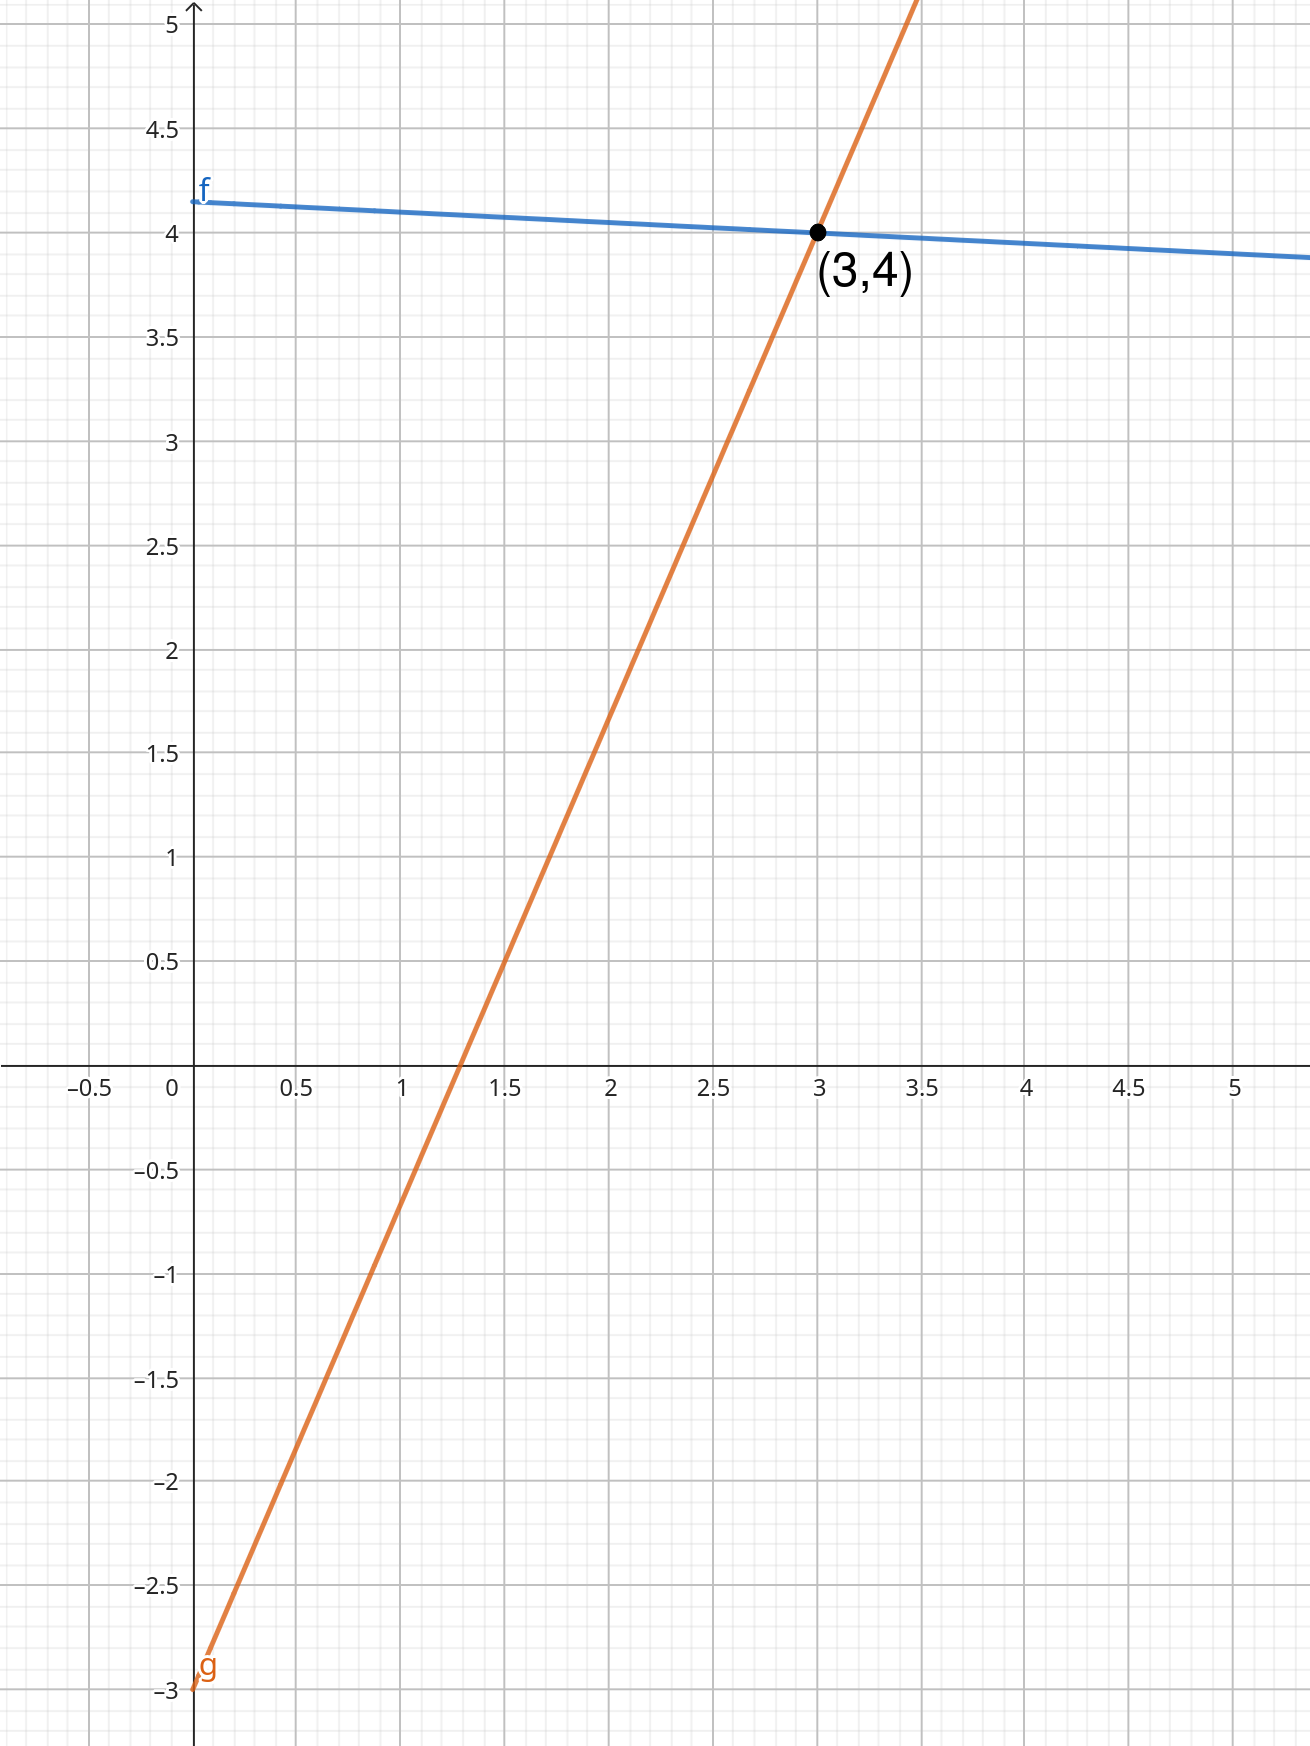
\includegraphics{01/actividad2/img/actividad2.png}\\
\end{align*}

\href{https://drive.google.com/file/d/1DXpY7xukQlkF4CswWKmvItGMWZuxZohS/view?usp=sharing}{Link} para el audio.
